\documentclass{article}
\usepackage{geometry}
\geometry{
  a4paper,
  margin=0.25in
}

\renewcommand\labelitemi{*}

% Packages
% ------------------
\usepackage{tkz-euclide}
\usepackage{tikz} % for drawing diagrams
\usepackage{bm} % bold mode
\usepackage{subfig}
\usepackage{graphicx}
%% \usepackage{amsfonts}
\usepackage{amssymb}
\usepackage{amsmath}
%% \usepackage{amsthm}
\usepackage{color}
\usepackage{algorithm}
\usepackage{algpseudocode}
\usepackage{dsfont}
\usepackage{forest}

% setup style of tikzlibrary elements
% ------------------------------------
\usetikzlibrary{patterns}
\usetikzlibrary{patterns.meta}
\usetikzlibrary{arrows}
\usetikzlibrary{quotes,angles}
\usetikzlibrary{positioning}
\usetikzlibrary{plotmarks}
\usetikzlibrary{math}
\usetikzlibrary{shapes.geometric, arrows}
\tikzstyle{block} = [rectangle, minimum width=2.5cm, minimum height=1cm, text centered, text width=2.7cm, draw=black, fill=white]
\tikzstyle{redblock} = [rectangle, thick, minimum width=2.5cm, minimum height=1cm, text centered, text width=2.7cm, draw=red, fill=white]
\tikzstyle{wideblock} = [rectangle, minimum width=2.5cm, minimum height=1cm, text centered, text width=5cm, draw=black, fill=white]
\tikzstyle{tallblock} = [rectangle, minimum width=1.9cm, minimum height=2cm, text centered, text width=1.9cm, draw=black, fill=white]
\tikzstyle{inputblock} = [rectangle, minimum width=1.7cm, minimum height=5cm, text centered, text width=1.7cm, draw=black, fill=white]
\tikzstyle{startstop} = [rectangle, rounded corners, minimum width=3cm, minimum height=1cm, text centered, draw=black, fill=white]
\tikzstyle{startstop_wide} = [rectangle, rounded corners, minimum width=6cm, minimum height=1cm, text centered, draw=black, fill=white]
\tikzstyle{io} = [trapezium, trapezium left angle=70, trapezium right angle=110, minimum width=3cm, minimum height=1cm, text centered, draw=black, fill=white]
\tikzstyle{process} = [rectangle, minimum width=4cm, minimum height=1cm, text centered, text width=4cm, draw=black, fill=white]
\tikzstyle{decision} = [diamond, minimum width=3cm, minimum height=1cm, text centered, draw=black, fill=white]
\tikzstyle{arrow} = [->,>=stealth] % can add "thick" to make it bold
\tikzset{radiation/.style={{decorate,decoration={expanding waves,angle=90,segment length=4pt}}}}

\tikzdeclarepattern{
  name=customdashed,
  bounding box={(-0.5pt,-0.5pt) and (10*1,1pt)},
  tile size={(10*1, 4pt)},
  tile transformation={},
  code={
    % Dash lengths (in pt or any TeX length)
    \draw[line width=0.4pt]
    (0pt,0pt) -- (20pt,0pt)
    (25pt,0pt) -- (38pt,0pt)
    (43pt,0pt) -- (48pt,0pt)
    (53pt,0pt) -- (85pt,0pt)
    (90pt,0pt) -- (100pt,0pt);
  }
}

%% new commands
% ------------------
\newcommand{\fixme}{\textcolor{red}{\textbf{fix me}} \space}
\newcommand{\attention}[1]{\noindent \fixme \textcolor{red}{#1}}

% \definecolor{light-gray}{gray}{0.95}
% \newcommand{\code}[1]{\colorbox{light-gray}{\texttt{#1}}}


\begin{document}


% @@@@@@@@@@@@@@@@@@@@@@@@@@@@@@@@@@@@@@@@@@@@@@@@@@

\begin{figure}[h]
\begin{center}
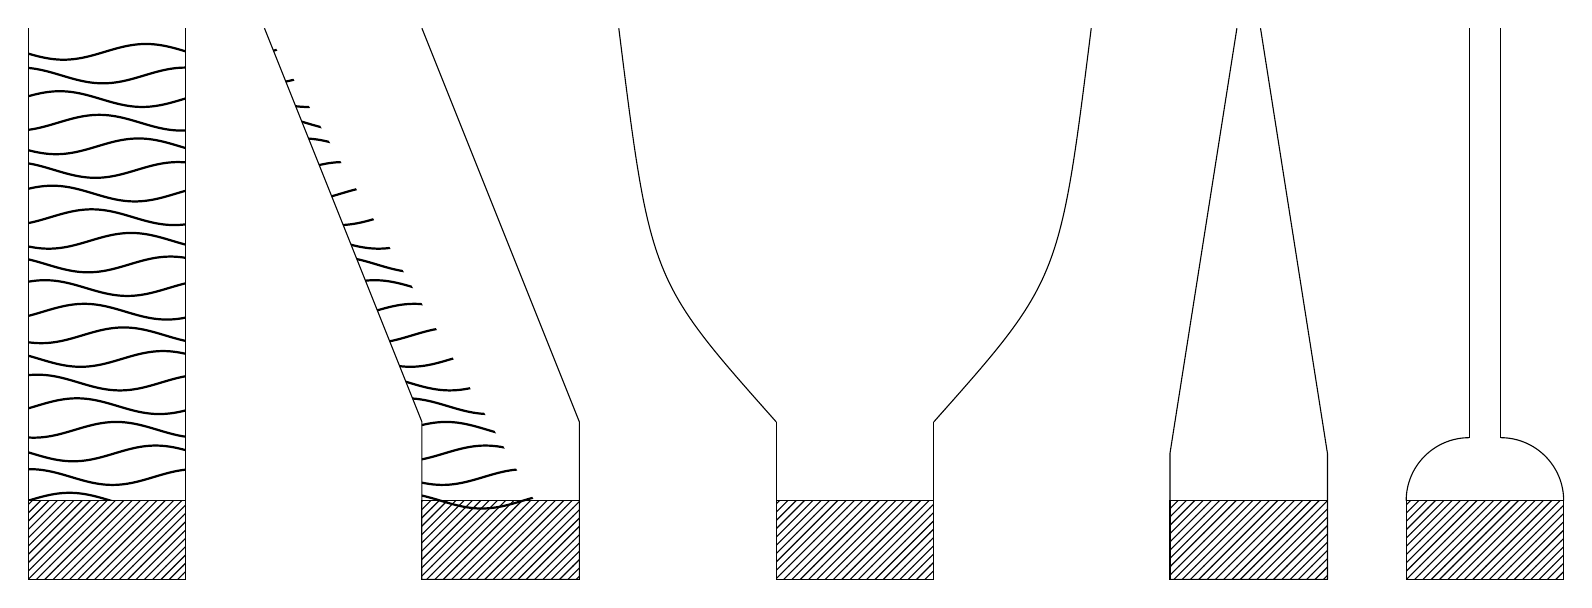
\begin{tikzpicture}[auto, node distance=2.7cm, >=latex']

  \tikzmath{\xmax = 20; \ymax = 7; \width = 2; \bh = 1;}
  \tikzmath{\cw1 = \width;}
  \tikzmath{\d = 0.15; \cw2 = \width*0.5 - \d;}

  \tikzmath{\s2 = \width + 1;}
  \tikzmath{\s3 = \width*3 + 1.5;}
  \tikzmath{\s4 = \s3+\cw1*2+\width+2 - \d;}
  \tikzmath{\s5 = \s4 + \d + 3;}

  % % comment out
  % \draw[step=1cm,gray,very thin] (0,0) grid (\xmax,\ymax);

  % Fig 1
  \draw (0,\ymax) -- (0,\bh) -- (\width,\bh) -- (\width,\ymax);
  \draw (0,0) rectangle +(\width,\bh);
  \draw[pattern={north east lines}] (0,0) rectangle +(\width,\bh);
  \begin{scope}
    \tikzmath{\width = 2;}
    \clip (0,\ymax) -- (0,\bh) -- (\width,\bh) -- (\width,\ymax);

    % \draw[thick, decorate, decoration={snake, amplitude=0.2mm, segment length=3mm}]

    \foreach \y in {0, 0.3, ..., 6} {
      \draw[thick]
      plot[domain=0:\width, smooth, samples=50]
      (\x, {1+sin(3*\x r + \y*5 r)*0.1 + \y});
    }
  \end{scope}

  % Fig 2
  \draw (\s2,\ymax) -- (\s2+\width,\bh*2) -- (\s2+\width,0) -- (\s2+\width*2,0);
  % \fill[pattern=customdashed] (\s2,\ymax) -- (\s2+\width,\bh*2) -- (\s2+\width,0) -- (\s2+\width*2,0);
  \draw (\s2+\width*2,0) -- (\s2+\width*2,\bh*2) -- (\s2+\width,\ymax);
  \draw[pattern={north east lines}] (\s2+\width,0) rectangle +(\width,\bh);
  \begin{scope}
    % \tikzmath{\width = 2; \s2 = \width + 1; \bh = 1;}
    \clip (\s2,\ymax) -- (\s2+\width,\bh*2) -- (\s2+\width,0) -- (\s2+\width*2,0);

    \foreach \y in {0, 0.3, ..., 6} {
      \draw[thick]
      plot[domain=0:5, smooth, samples=50]
      (\x+\s2, {1+sin(3*(\x+\s2) r + \y*5 r)*0.1 + \y});
    }
  \end{scope}

  % Fig 3
  \tikzmath{\c = 0.7; \cx = 0.1; \cy1 = (\ymax + \bh*2) / 2 - \c;}
  \draw (\s3,\ymax) .. controls (\s3+0.5-\cx,\cy1) .. (\s3+\cw1,\bh*2);
  \draw (\s3+\cw1,\bh*2) -- (\s3+\cw1,0) -- (\s3+\cw1+\width,0) -- (\s3+\cw1+\width,\bh*2);
  \draw (\s3+\cw1+\width,\bh*2) .. controls (\s3+\cw1+\width+1.5+\cx,\cy1) .. (\s3+\cw1*2+\width,\ymax);
  \draw[pattern={north east lines}] (\s3+\cw1,0) rectangle +(\width,\bh);

  % Fig 4
  \tikzmath{\m = 1.6;}
  \draw (\s4,\ymax) -- (\s4-\cw2,\bh*\m) -- (\s4-\cw2,0) -- (\s4-\cw2+\width,0);
  \draw (\s4-\cw2+\width,0) -- (\s4-\cw2+\width,\bh*\m) -- (\s4+\d*2,\ymax);
  \draw[pattern={north east lines}] (\s4-\cw2,0) rectangle +(\width,\bh);

  % Fig 5
  % \draw(\s5,\ymax) -- (\s5,\bh*2);
  \draw (\s5-1,\bh) arc (180 : 90 : 0.8cm);
  \draw (\s5-1,\bh) -- (\s5-1,0) -- (\s5-1+\width,0) -- (\s5-1+\width,\bh);
  \draw (\s5-1+\width,\bh) arc (0 : 90 : 0.8cm);
  \draw(\s5-1+0.8,\ymax) -- (\s5-1+0.8,\bh*1.8);
  \draw(\s5-1+1.2,\ymax) -- (\s5-1+1.2,\bh*1.8);
  \draw[pattern={north east lines}] (\s5-1,0) rectangle +(\width,\bh);


\end{tikzpicture}
\end{center}
 \caption{Duhem-1905N,fig-1}
\label{fig:Duhem-fig1}
\end{figure}

% @@@@@@@@@@@@@@@@@@@@@@@@@@@@@@@@@@@@@@@@@@@@@@@@@@


\begin{figure}[h]
\begin{center}
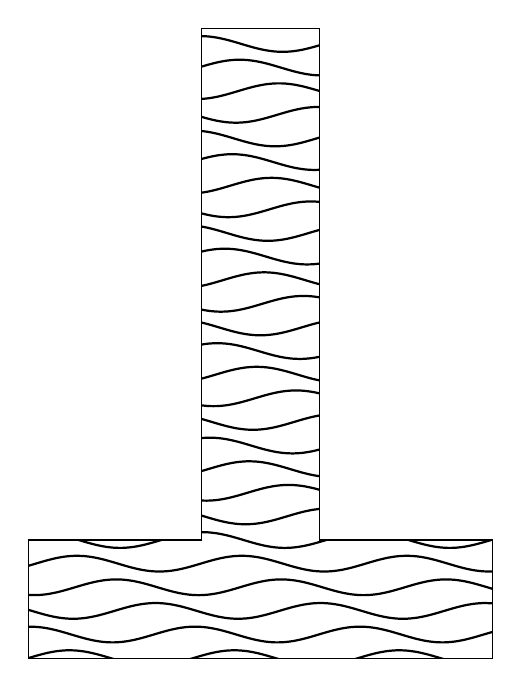
\begin{tikzpicture}[auto, node distance=2.7cm, >=latex']

  \tikzmath{\xmax = 20; \ymax = 8;}
  % % comment out
  % \draw[step=1cm,gray,very thin] (0,0) grid (\xmax,\ymax);

  % Fig 1
  \begin{scope}
    \tikzmath{\w = 2.2; \h = 1.5; \tw = 1.5;}
    \tikzmath{\maxw = 2*\w+\tw;}

    \draw (0,0) -- (0,\h) -- (\w,\h) -- (\w,\ymax) -- (\w+\tw,\ymax) -- (\w+\tw,\h) -- (\maxw,\h) -- (\maxw,0) -- (0,0);
    \clip (0,0) -- (0,\h) -- (\w,\h) -- (\w,\ymax) -- (\w+\tw,\ymax) -- (\w+\tw,\h) -- (\maxw,\h) -- (\maxw,0) -- (0,0);

    \foreach \y in {0, 0.3, ..., \ymax} {
      \draw[thick]
      plot[domain=0:\maxw, smooth, samples=50]
      (\x, {sin(3*\x r + \y*5 r)*0.1 + \y});
    }
  \end{scope}

  % % Fig 2
  % \begin{scope} []
  % \end{scope}

\end{tikzpicture}
\end{center}
 \caption{Duhem-1905N,fig-2}
\label{fig:Duhem-fig2}
\end{figure}

% @@@@@@@@@@@@@@@@@@@@@@@@@@@@@@@@@@@@@@@@@@@@@@@@@@

% \section{2025.05}
% ---------------------------

\begin{figure}[h]
\begin{center}
\begin{tikzpicture}[auto, node distance=2.7cm, >=latex']

  \tikzmath{\ymax = 16; \b = 1; \tmax = 11;}

  % % comment out
  % \draw[step=1cm,gray,very thin] (0,0) grid (10,\ymax);

  \draw (1,\b) -- (1,\ymax) -- (2,\ymax) -- (2,\b+1);
  \draw (1,\b) arc (180 : 270 : 1cm) node[below left]{C};
  \draw (2,\b+1) arc (180 : 270 : 1cm);

  \draw (2,\b-1) -- (7,\b-1);
  \draw (7,\b-1) arc (270 : 360 : 1cm);

  \draw (3,\b) -- (6,\b);
  \draw (6,\b) arc (270 : 360 : 1cm);

  \draw (7,\b+1) -- (7,\b+2) node[above right]{I};
  \draw (7,\b+2) arc (270 : 180 : 2cm);

  \draw (8,\b) -- (8,\b+2) node[below right]{D};
  \draw (8,\b+2) arc (270 : 360 : 2cm);

  \draw (5,\b+4) -- (5,\tmax) node[left]{E} -- (10,\tmax) node[right]{F} -- (10,\b+4);
  \draw (5,7) -- (5,8) node[left]{C} -- (10,8) node[right]{H} -- (10,7) -- (5,7) node[left]{Q};
  \draw (1,8) node[left]{L} -- (2,8);
  \draw (1,\ymax-3) node[left]{A} -- (2,\ymax-3) node[right]{B};

\end{tikzpicture}
\end{center}
 \caption{Duhem-1905N,fig-4}
\label{fig:Duhem-fig4}
\end{figure}


% @@@@@@@@@@@@@@@@@@@@@@@@@@@@@@@@@@@@@@@@@@@@@@@@@@



% -----------------------------
%% \bibliography{references}


% -----------------------------
\end{document}

%%% Local Variables:
%%% mode: latex
%%% TeX-master: t
%%% End:
